\chapter{Undecidability and Computability}\label{ch:undecidability}

Propositional validity is decidable by truth tables, and first-order validity is
semi-decidable by proof search. Is there an algorithm that decides first-order validity
outright? Hilbert's \emph{Entscheidungsproblem} (1928) asked exactly this. Church and
Turing (1936) independently showed the answer is \emph{no}. To prove such a thing we need
a precise definition of ``algorithm''.

\section{Turing machines}

\begin{definition}[Turing machine]
A (deterministic) \emph{Turing machine} consists of
\begin{itemize}
  \item a finite set of states $Q$, with a start state $q_0$ and halting states
        (e.g.\ $q_{\mathrm{accept}}$, $q_{\mathrm{reject}}$);
  \item a tape alphabet $\Gamma$ including a blank symbol $\sqcup$, and an input alphabet
        $\Sigma\subseteq\Gamma\setminus\{\sqcup\}$;
  \item a transition function
        $\delta: Q\times\Gamma\to Q\times\Gamma\times\{L,R\}$.
\end{itemize}
The machine has an infinite tape, initially holding the input followed by blanks, and a
head on the leftmost cell. At each step, in state $q$ reading symbol $a$, if
$\delta(q,a)=(q',b,D)$ it writes $b$, moves one cell in direction $D$, and enters $q'$. It
stops when it enters a halting state; it may also run forever.
\end{definition}

\begin{center}
\begin{tikzpicture}[>=Stealth,x=0.75cm,font=\small]
  \foreach \s [count=\k from 0] in {1,0,1,1,{$\sqcup$},{$\sqcup$},{$\sqcup$}}
    \node[draw,minimum width=0.75cm,minimum height=0.7cm] at (\k,0) {\s};
  \node at (7.2,0) {$\cdots$};
  \node[draw,rounded corners,fill=blue!8] (ctl) at (2,-1.6) {finite control: state $q$};
  \draw[->,thick] (ctl.north) -- (2,-0.4);
  \node[font=\scriptsize,anchor=west] at (7.7,0) {tape, infinite to the right};
\end{tikzpicture}

\small A configuration: tape contents, head position (here on the third cell) and current state.
\end{center}

\begin{example}
A machine that accepts binary strings with an even number of $1$s scans right, toggling
between states $q_{\mathrm{even}}$ and $q_{\mathrm{odd}}$ on each $1$, and on reaching
the blank accepts iff it is in $q_{\mathrm{even}}$. (This one does not even need to write;
machines that use the tape as memory can do far more, e.g.\ recognise
$\{0^n1^n : n\ge0\}$ by repeatedly crossing off a $0$ and a matching $1$.)
\end{example}
\begin{center}
\begin{tikzpicture}[shorten >=1pt,node distance=3.2cm,on grid,auto,>=Stealth,
  every state/.style={minimum size=1.1cm,font=\small}]
  \node[state,initial] (e) {$q_{\mathrm{even}}$};
  \node[state] (o) [right=of e] {$q_{\mathrm{odd}}$};
  \node[state,accepting] (a) [below=2cm of e] {acc};
  \node[state] (r) [below=2cm of o] {rej};
  \path[->]
    (e) edge[loop above] node {$0/0,R$} ()
    (e) edge[bend left] node {$1/1,R$} (o)
    (o) edge[bend left] node {$1/1,R$} (e)
    (o) edge[loop above] node {$0/0,R$} ()
    (e) edge node[swap] {$\sqcup/\sqcup,R$} (a)
    (o) edge node {$\sqcup/\sqcup,R$} (r);
\end{tikzpicture}

\small Edge label $a/b,D$: reading $a$, write $b$ and move in direction $D$.
\end{center}

\begin{important}[Church--Turing thesis]
Every function that is computable by an effective procedure (an ``algorithm'' in the
intuitive sense) is computable by a Turing machine. This is not a theorem (``effective
procedure'' is informal) but is supported by the fact that all proposed models (lambda
calculus, recursive functions, register machines, real programming languages) compute
exactly the same functions.
\end{important}

So we may reason about ``programs'' in any language (say, C or Racket) instead of Turing
machines. Crucially, programs are finite strings, so they can be given as \emph{input} to
other programs; a \emph{universal} Turing machine (an interpreter) can simulate any machine
given its description.

\section{Decision problems}

\begin{definition}
A \emph{decision problem} is a yes/no question about inputs, i.e.\ a set $L$ of strings
(the ``yes'' instances).
\begin{itemize}
  \item $L$ is \emph{decidable} (recursive) if some program halts on every input and
        answers ``yes'' exactly on members of $L$.
  \item $L$ is \emph{semi-decidable} (recursively enumerable) if some program halts with
        ``yes'' exactly on members of $L$ (and may loop forever on non-members).
\end{itemize}
\end{definition}

\begin{theorem}
$L$ is decidable iff both $L$ and its complement are semi-decidable.
\end{theorem}
\begin{proof}
($\Leftarrow$) Run both semi-deciders in parallel (alternating steps); exactly one halts.
($\Rightarrow$) A decider is a semi-decider for $L$, and swapping its answers gives one for
the complement.
\end{proof}

\section{The halting problem}

\begin{definition}
$\textsc{Halt}=\{(P,x) : \text{program } P \text{ halts on input } x\}$.
\end{definition}

$\textsc{Halt}$ is semi-decidable: simulate $P$ on $x$ and say ``yes'' if it halts.

\begin{theorem}[Turing 1936]
$\textsc{Halt}$ is undecidable.
\end{theorem}
\begin{proof}
Suppose a program \code{halts(P, x)} always terminates and returns true iff $P$ halts on
$x$. Build:
\begin{lstlisting}[style=c]
void diag(Program P) {
    if (halts(P, P))     // would P halt when given its own code?
        while (1) { }    // ... then loop forever
    else
        return;          // ... otherwise halt
}
\end{lstlisting}
Consider \code{diag(diag)}. If it halts, then \code{halts(diag, diag)} returned true, so
\code{diag} enters the infinite loop and does not halt. If it does not halt, then
\code{halts(diag, diag)} returned false, so \code{diag} returns, i.e.\ halts. Either way
we have a contradiction, so \code{halts} cannot exist.
\end{proof}

This is a \emph{diagonal argument}, the same idea as Cantor's proof that $\R$ is
uncountable and as the liar paradox ``this sentence is false''.
Picture a table of every program's behaviour on every program as input; \code{diag}
is built to disagree with the diagonal, so it cannot be any row of the table:
\begin{center}
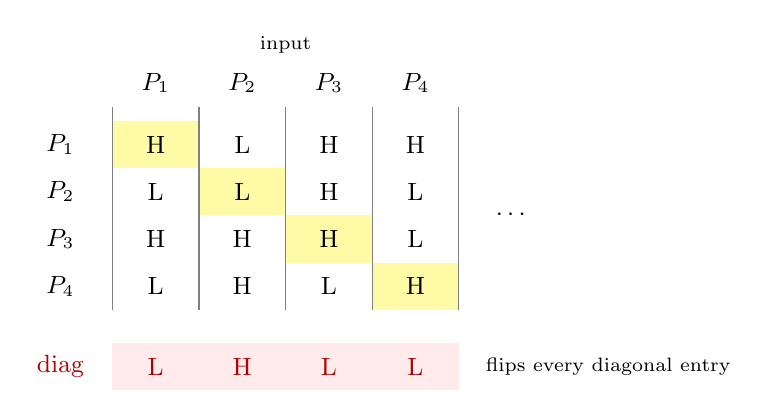
\begin{tikzpicture}[x=1.1cm,y=0.6cm,font=\small]
  \foreach \c [count=\i] in {$P_1$,$P_2$,$P_3$,$P_4$} \node at (\i,0.8) {\c};
  \node[font=\scriptsize] at (2.5,1.6) {input};
  \foreach \r/\vals [count=\j] in {{$P_1$}/{H,L,H,H},{$P_2$}/{L,L,H,L},{$P_3$}/{H,H,H,L},{$P_4$}/{L,H,L,H}} {
    \node at (-0.1,-\j+0.5) {\r};
    \foreach \v [count=\i] in \vals {
      \ifnum\i=\j \fill[yellow!35] (\i-0.5,-\j) rectangle (\i+0.5,-\j+1); \fi
      \node at (\i,-\j+0.5) {\v};
    }
  }
  \foreach \x in {0.5,1.5,2.5,3.5,4.5} \draw[gray] (\x,-4) -- (\x,0.3);
  \node at (5.1,-2) {$\cdots$};
  \node[red!70!black] at (-0.1,-5.2) {\code{diag}};
  \foreach \v [count=\i] in {L,H,L,L} {\fill[red!8] (\i-0.5,-5.7) rectangle (\i+0.5,-4.7); \node[red!70!black] at (\i,-5.2) {\v};}
  \node[font=\scriptsize,anchor=west] at (4.7,-5.2) {flips every diagonal entry};
\end{tikzpicture}

\small H $=$ halts, L $=$ loops. Row $i$, column $j$: what $P_i$ does on input $P_j$.
\end{center}

\begin{corollary}
The complement of $\textsc{Halt}$ is not even semi-decidable.
\end{corollary}

\section{Reductions}

\begin{definition}
A problem $A$ \emph{reduces} to $B$ ($A\le B$) if there is a computable function $f$ with
$x\in A\iff f(x)\in B$ for all $x$.
\end{definition}

If $A\le B$ and $B$ is decidable, then $A$ is decidable (compute $f(x)$, then run $B$'s
decider). Contrapositively:

\begin{important}[Proving undecidability]
To show $B$ undecidable, reduce a known undecidable problem (usually $\textsc{Halt}$)
\emph{to} $B$: show that a decider for $B$ would give a decider for $\textsc{Halt}$.
The direction matters: reducing $B$ to $\textsc{Halt}$ proves nothing about $B$'s
hardness.
\end{important}

\begin{center}
\begin{tikzpicture}[>=Stealth,font=\small,box/.style={draw,rounded corners,fill=blue!5,minimum height=0.9cm,align=center}]
  \node (x) at (0,0) {$x$};
  \node[box] (f) at (2.2,0) {compute\\ $f(x)$};
  \node[box,fill=green!8] (d) at (5.6,0) {decider\\ for $B$};
  \node (out) at (8.6,0) {yes / no};
  \draw[->] (x) -- (f); \draw[->] (f) -- node[above,font=\scriptsize]{$f(x)$} (d);
  \draw[->] (d) -- (out);
  \draw[dashed,rounded corners] (1.1,-0.9) rectangle (6.7,1.05);
  \node[font=\scriptsize,anchor=south west] at (1.1,1.05) {a decider for $A$ (impossible if $A$ is undecidable)};
\end{tikzpicture}
\end{center}

\begin{example}[Halting on empty input]
$\textsc{Halt}_\varepsilon=\{P : P \text{ halts on empty input}\}$ is undecidable. Given
$(P,x)$, construct $P_x$: ``ignore your input and run $P$ on $x$''. Then $P_x$ halts on
the empty input iff $P$ halts on $x$. The map $(P,x)\mapsto P_x$ is computable, so
$\textsc{Halt}\le\textsc{Halt}_\varepsilon$.
\end{example}

\begin{example}[Program equivalence]
$\textsc{Equiv}=\{(P,Q): P,Q \text{ compute the same function}\}$ is undecidable. Reduce
$\textsc{Halt}_\varepsilon$: given $P$, build $P'$: ``run $P$ on empty input, then return
$0$'' and $Q$: ``return $0$''. Then $P'\equiv Q$ iff $P$ halts on empty input.
\end{example}

\begin{aside}
\textbf{Rice's theorem} generalises these: every non-trivial property of the
\emph{function} computed by a program (``does it ever output 7?'', ``is it total?'',
``does it compute factorial?'') is undecidable. So no compiler or static analyser can
perfectly decide such questions; real tools are sound-but-incomplete approximations. This
is also why the verification in Chapter~\ref{ch:hoare} needs human-supplied invariants.
\end{aside}

\section{Undecidability of first-order logic}

\begin{theorem}[Church 1936, Turing 1936]
The set of valid sentences of first-order logic (in a language with at least one binary
predicate symbol) is undecidable.
\end{theorem}
\begin{proof}[Proof idea]
Reduce $\textsc{Halt}$ (or the Post correspondence problem) to validity. Given a machine $M$
and input $x$, build a sentence $\varphi_{M,x}$ whose axioms describe $M$'s configurations
and transitions, using predicates like $\mathit{State}_q(t)$, $\mathit{Head}(t,c)$,
$\mathit{Sym}_a(t,c)$ (``at time $t$ the head is on cell $c$'', etc.), with conclusion
``at some time a halting state is reached''. Then $\models\varphi_{M,x}$ iff $M$ halts on
$x$. A validity decider would decide $\textsc{Halt}$.
\end{proof}

\begin{important}[Decidability landscape]
\begin{center}
\begin{tabular}{ll}
\toprule
Problem & Status\\
\midrule
Propositional validity / satisfiability & decidable (co-NP / NP-complete)\\
First-order validity & semi-decidable, not decidable\\
First-order satisfiability & not semi-decidable (co-semi-decidable)\\
Monadic FOL (unary predicates only) & decidable\\
Presburger arithmetic ($\N$ with $+$) & decidable\\
True arithmetic ($\N$ with $+,\cdot$) & not even semi-decidable\\
\bottomrule
\end{tabular}
\end{center}
\end{important}

\begin{center}
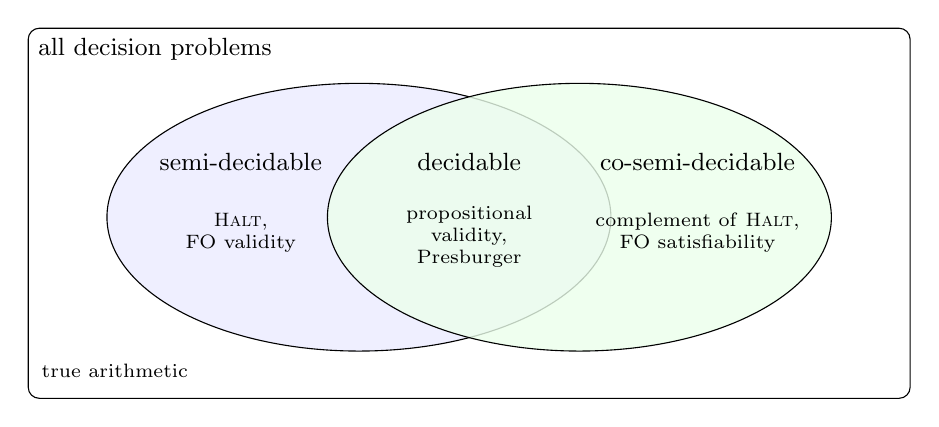
\begin{tikzpicture}[font=\scriptsize]
  \draw[rounded corners] (-5.6,-2.4) rectangle (5.6,2.3);
  \node[anchor=north west,font=\small] at (-5.6,2.3) {all decision problems};
  \draw[fill=blue!8,fill opacity=0.8] (-1.4,-0.1) ellipse (3.2cm and 1.7cm);
  \draw[fill=green!8,fill opacity=0.8] (1.4,-0.1) ellipse (3.2cm and 1.7cm);
  \node[font=\small] at (-2.9,0.6) {semi-decidable};
  \node[font=\small] at (2.9,0.6) {co-semi-decidable};
  \node[font=\small] at (0,0.6) {decidable};
  \node[align=center] at (0,-0.35) {propositional\\ validity,\\ Presburger};
  \node[align=center] at (-2.9,-0.3) {\textsc{Halt},\\ FO validity};
  \node[align=center] at (2.9,-0.3) {complement of \textsc{Halt},\\ FO satisfiability};
  \node[align=center] at (-4.5,-2.05) {true arithmetic};
\end{tikzpicture}
\end{center}

\section{G\"odel's incompleteness theorems}

\begin{definition}
A set of axioms $\Gamma$ is
\begin{itemize}
  \item \emph{consistent} if it does not prove both $\varphi$ and $\neg\varphi$;
  \item \emph{complete} if for every sentence $\varphi$, it proves $\varphi$ or proves
        $\neg\varphi$;
  \item \emph{effectively axiomatised} if there is an algorithm that decides whether a
        given sentence is an axiom (e.g.\ PA, with its induction scheme).
\end{itemize}
(Do not confuse completeness of a \emph{theory} with completeness of a \emph{proof
system}: G\"odel proved the latter in 1929 and the failure of the former in 1931.)
\end{definition}

\begin{theorem}[First incompleteness theorem]
Any consistent, effectively axiomatised theory that can express basic arithmetic (e.g.\
PA) is incomplete: there is a sentence $G$ such that neither $G$ nor $\neg G$ is
provable. If the theory is sound for $\N$, then $G$ is true in $\N$ but unprovable.
\end{theorem}

\paragraph{Idea.}
\begin{enumerate}
  \item \emph{G\"odel numbering}: encode symbols, formulas and proofs as natural numbers,
        so statements about syntax become statements about numbers.
  \item Show ``$p$ is the code of a proof of the formula with code $n$'' is expressible
        by an arithmetic formula $\mathit{Prf}(p,n)$, and let
        $\mathit{Prov}(n)\equiv\exists p\,\mathit{Prf}(p,n)$.
  \item \emph{Diagonal lemma}: build a sentence $G$ with
        $\vdash G\leftrightarrow\neg\mathit{Prov}(\ulcorner G\urcorner)$, i.e.\ $G$ says
        ``I am not provable''.
  \item If $G$ were provable, then $G$ would be false while provable (inconsistency, or
        unsoundness). So $G$ is unprovable, and hence true.
\end{enumerate}

\paragraph{Computability view.} If true arithmetic had a complete effective
axiomatisation, we could decide truth in $\N$ by enumerating all proofs until one of
$\varphi$ or $\neg\varphi$ appears. But the halting problem is expressible in arithmetic
(``$\exists t$: $M$ halts on $x$ within $t$ steps''), so this would decide
$\textsc{Halt}$. Contradiction. This gives a quick proof of a version of the first
theorem.

\begin{theorem}[Second incompleteness theorem]
A consistent, effectively axiomatised theory containing enough arithmetic cannot prove
its own consistency (the sentence $\neg\mathit{Prov}(\ulcorner 0=s(0)\urcorner)$).
\end{theorem}

\begin{aside}
Consequences: there is no ``final'' axiom system for mathematics; Hilbert's programme of
proving the consistency of mathematics by finitary means cannot be carried out in full.
Concrete true-but-unprovable statements in PA include Goodstein's theorem and the
Paris--Harrington theorem.
\end{aside}

\section*{Summary}
\begin{itemize}
  \item Turing machines formalise ``algorithm''; the Church--Turing thesis says they
        capture all effective computation.
  \item Decidable: always halts with the right answer; semi-decidable: halts on yes
        instances.
  \item The halting problem is undecidable (diagonalisation); prove other problems
        undecidable by reducing $\textsc{Halt}$ to them.
  \item First-order validity is semi-decidable but undecidable (Church--Turing).
  \item G\"odel: any consistent, effective theory of arithmetic is incomplete and cannot
        prove its own consistency.
\end{itemize}
